%!TEX root = ../thesis_phd.tex
%%%%%%%%%%%%%%%%%%%%%%%%%%%%%%%%%%%%%%%%%%%%%%%%%%%%%%%%%%%%%%%%%%%%%%%%%%%%%%%%
% experiment.tex: Chapter describing the experiment
%%%%%%%%%%%%%%%%%%%%%%%%%%%%%%%%%%%%%%%%%%%%%%%%%%%%%%%%%%%%%%%%%%%%%%%%%%%%%%%%
\chapter{\nova}
\label{nova_chapter}
Neutrinos at the Main Injector (\numi) is a high-intensity neutrino source located at Fermilab.  The \numi Off-axis \nue Appearance (\nova) experiment will employ this source in one of the latest efforts in the class of long baseline neutrino experiments.  Long baseline neutrino experiments aim to observe neutrino oscillations in a detector placed at some long distance -- known as the baseline -- from a neutrino source.  \nova employs two detectors for observation of neutrinos, one near the source and another 810 km away in Ash River, Minnesota.  The Near Detector (ND) is used to observe the initial  \numi flux at a distance where oscillations are negligible; the Far Detector (FD) observes the \numi flux subject to neutrino oscillations.  \numi will be discussed in section~\ref{sec:numi}, the detectors in \ref{sec:detectors} and \nova's physics goals in \ref{goals}. 

\section{\numi and  Off-axis Alignment }\label{sec:numi}

In a process similar to the Brookhaven experiment that discovered the muon neutrino, the \numi beam is generated by protons accelerated to 120 GeV by the Main Injector at Fermilab.  These protons are steered into a graphite target producing a shower of hadrons including pions and kaons.  A schematic of the \numi configuration can be seen in Figure~\ref{numi}.  Particles in the hadronic shower are focused into a beam by the magnetic field created in ``focusing horns.''    Muon neutrinos are then produced when charged pions decay as shown in \eqref{pions}.  Alternatively, antiparticles can be focused by switching the direction of the electric current in the focusing horns, and as a result, \numi can serve as either a neutrino or antineutrino beam.  As opposed to pions which yield muon neutrinos 99.98\% of their decays, electron neutrinos produced in muon and kaon decay are an irreducible background in electron neutrino analyses.  The muons produced in pion decay are absorbed in rock upstream of the \nova Near Detector, eliminating them as background.  Upon upgrades scheduled for completion in 2013, \numi will boast an intensity of 700 kW, delivering bunches of $4.9 \times 10^{13}$ protons to the target every 1.3 seconds.\cite{tdr}

\begin{figure}[t]
  \begin{center}
    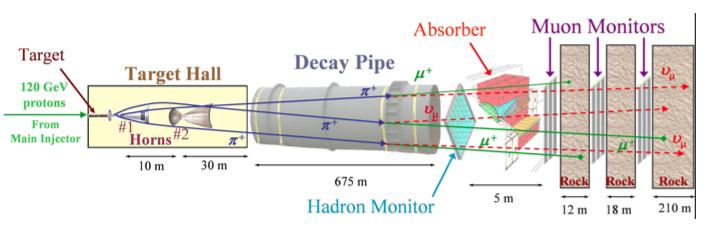
\includegraphics[width=\textwidth]{figures/figures/numi.png}
  \end{center}
  \caption[A schematic of the \numi neutrino source.]{A schematic of the \numi neutrino source.  Courtesy of Robert Zwaska \cite{zwaska2005thesis}.}
  \label{numi}
\end{figure}

Rather than being placed directly in the \numi beam line, the \nova detectors are placed 14.6 milliradians off of the beam axis.  
\begin{figure}[t]
\centering
\begin{subfigure}[c]{0.47\textwidth}
                \centering
                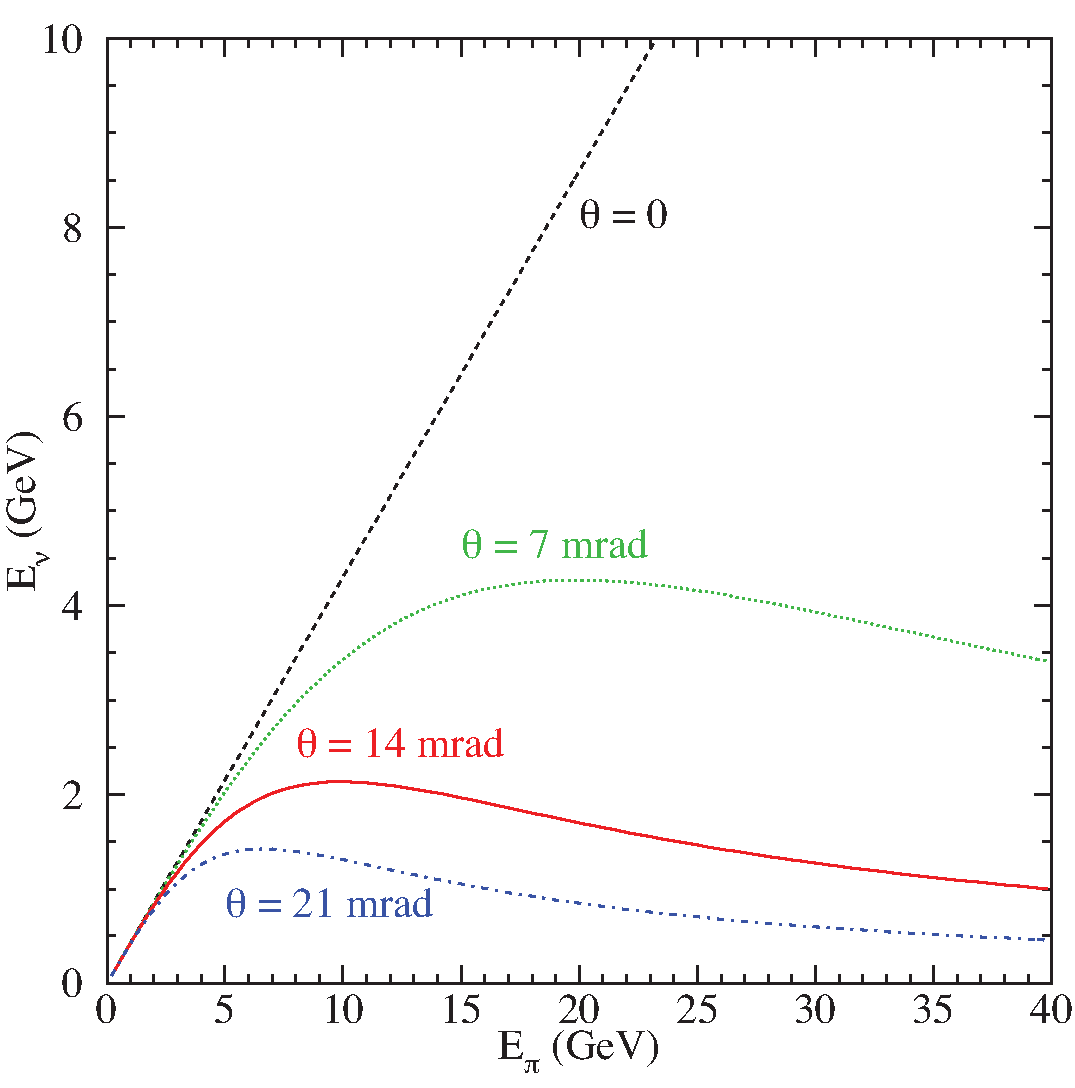
\includegraphics[width=\textwidth]{figures/plots/nova/EnuVsEpi.pdf}
                \caption{Neutrino energy vs. pion energy at various angles relative to the beam axis.}
                 \label{EnuEpi}
        \end{subfigure}
        ~
\begin{subfigure}[c]{0.47\textwidth}
                \centering
                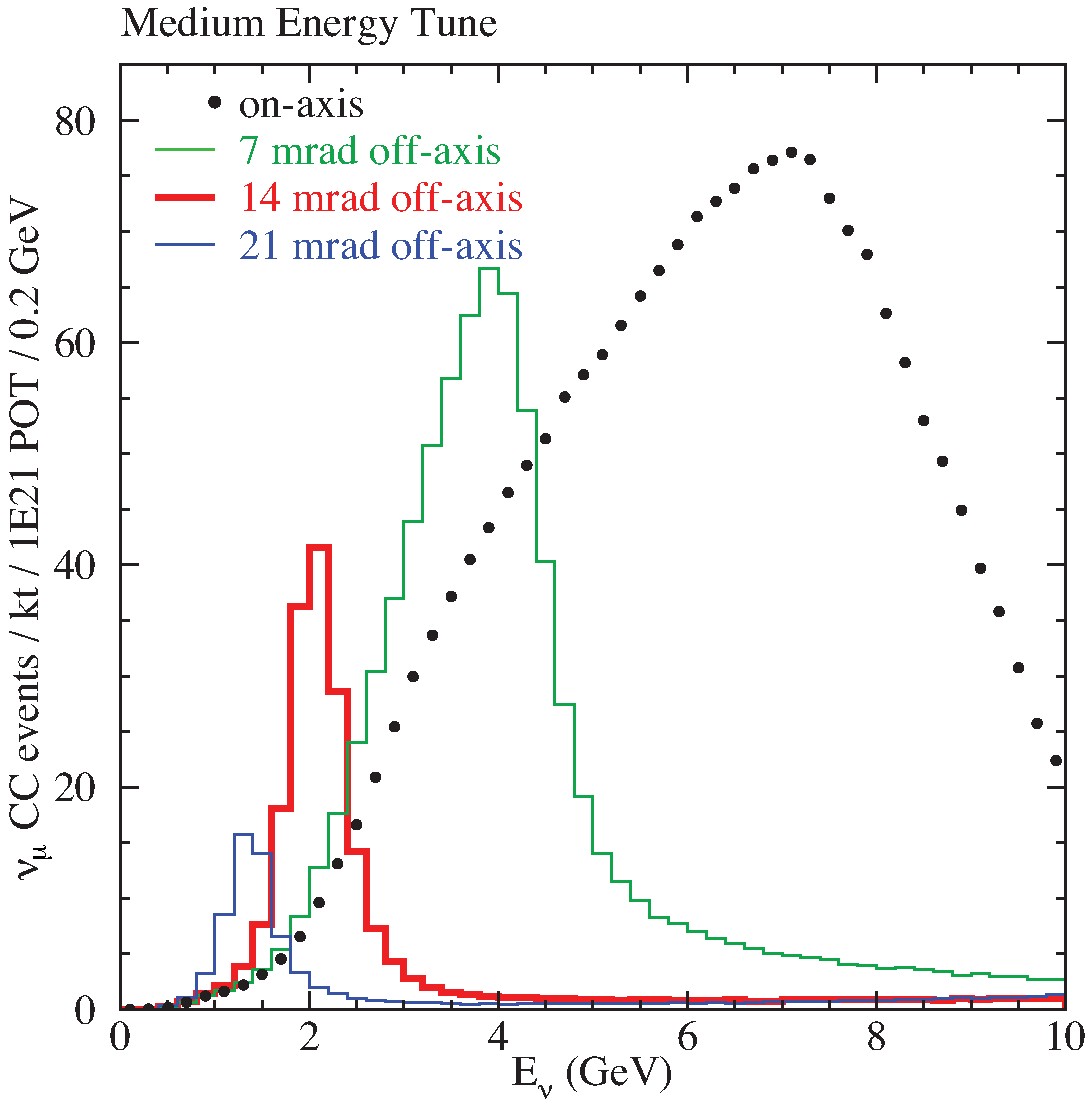
\includegraphics[width=\textwidth]{figures/plots/nova/energySpectrum.pdf}
                \caption{Expected \numu event counts vs. neutrino energy at various angles relative to the beam axis}
                \label{fluxEnu}

        \end{subfigure}
        \caption{Effects of off-axis design.}
\end{figure}As displayed in Figure~\ref{EnuEpi}, the neutrinos produced on axis demonstrate a strong dependence on the pion energy; on the other hand, the energy of neutrinos produced slightly off axis correlates weakly with pion energy.  Since the pions produced at the target have a spread of energies, this weak correlation helps narrow the neutrino energy spectrum, as seen in Figure~\ref{fluxEnu}.  The neutrino energy spectrum at 14.6 milliradians is characterized by a sharp peak near 2 GeV; there is a significant disappearance probability for neutrinos in this energy range at a baseline 810 km, the distance of the far detector.  Further, the narrowness of the peak reduces the fraction of the spectrum above 2 GeV.  Neutral current interactions produce diminished amounts of visible energy since much is carried away by the outgoing neutrino.  High energy neutral-current background events can be misidentified as charged-current signal events; the narrow energy peak helps reduce this background.  
 
\section{\nova Detectors}
\label{sec:detectors}
The \nova detectors are densely instrumented neutrino detectors designed for measurement of the probabilities $P(\nu_\mu \rightarrow \nu_\mu)$ and $P(\nu_\mu \rightarrow \nu_e)$.  Two detectors will be used to study these probabilities, one small Near Detector placed on the Fermilab grounds 1 km away from the \numi source and another Far Detector 810 km away in Ash River, Minnesota.  The detectors are designed to be functionally identical to each other; they are built with the same materials and geometry to constrain uncertainties due to variation in detector efficiency. 

\begin{figure}[t]
\begin{subfigure}[t]{0.25\textwidth}
                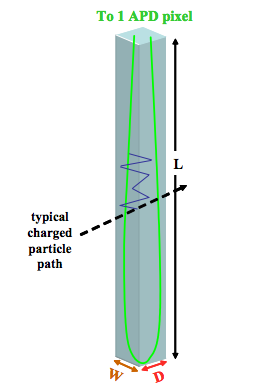
\includegraphics[height=0.35\textheight]{figures/figures/cell.png}
               \caption{A NO$\nu A$ cell.}
                 \label{cell}
        \end{subfigure}
        ~
\begin{subfigure}[t]{0.75\textwidth}
                \centering
                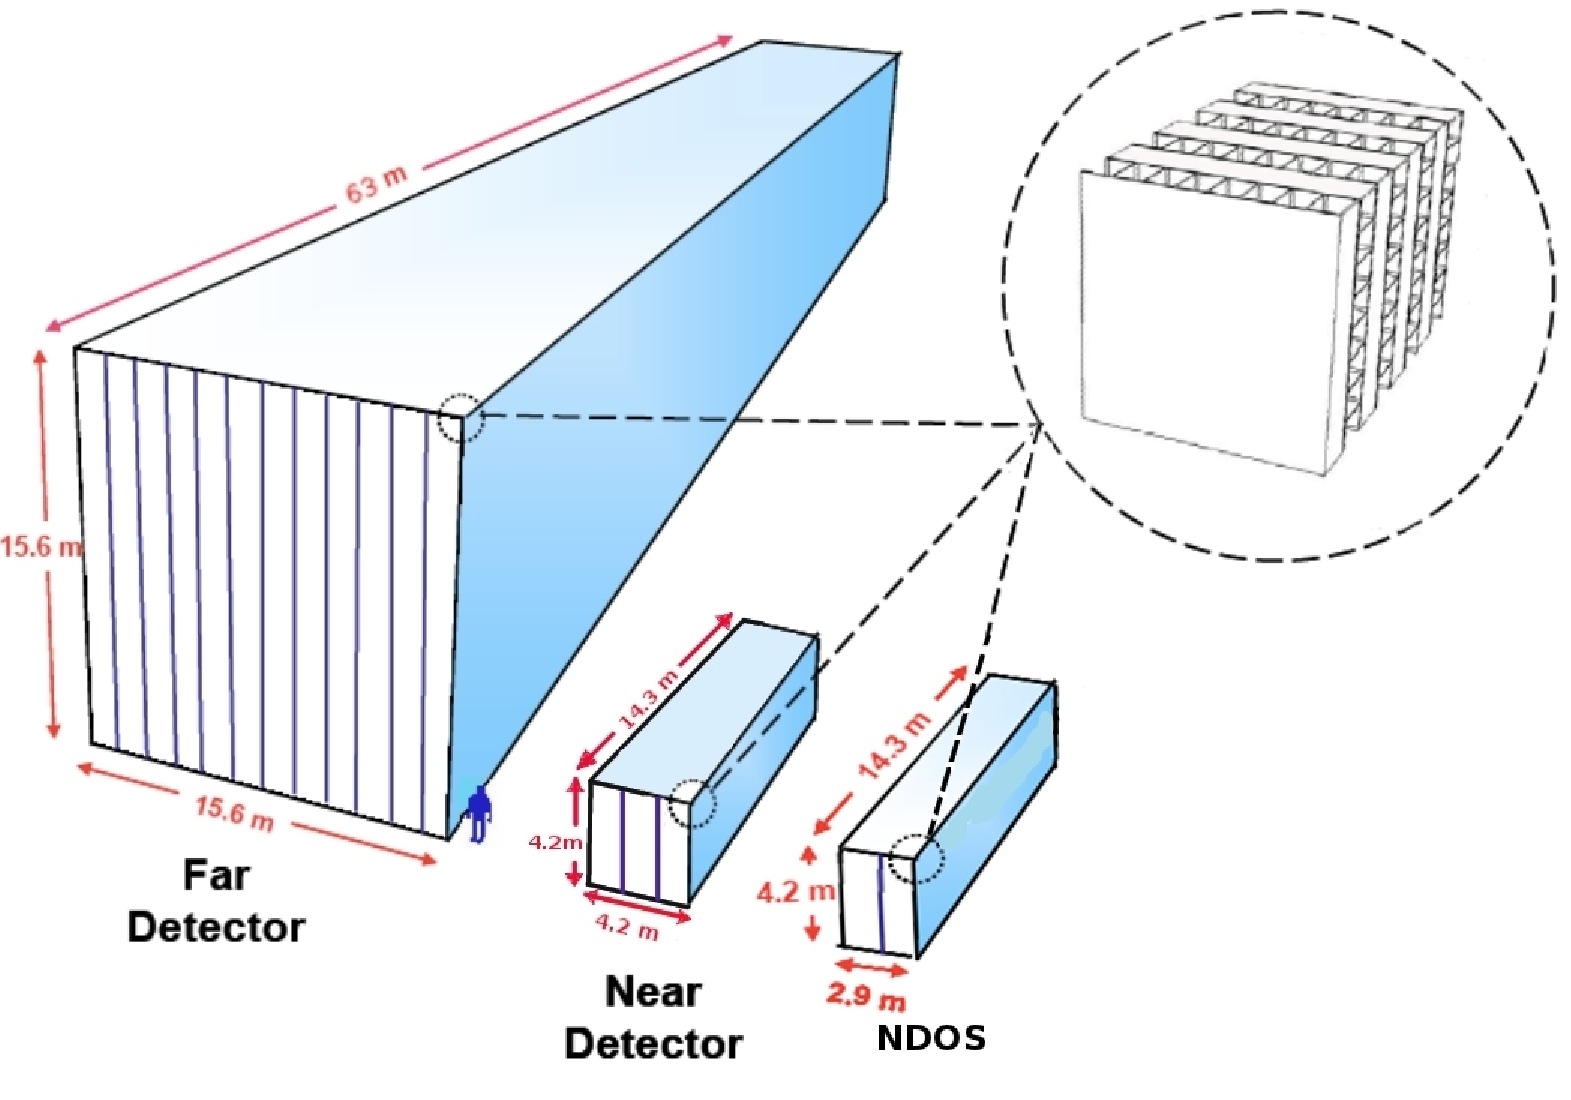
\includegraphics[height=0.35\textheight]{figures/figures/detectors.pdf}
               \caption{Scale and geometry of the \nova detectors.}
                \label{detector}

        \end{subfigure}
        \caption{}
\end{figure}

 A design goal of the experiment is to implement detectors that allow reconstruction of electromagnetic showers for measurement of $P(\nu_\mu \rightarrow \nu_e)$.  Electrons are difficult to detect in material with high density since they are quickly attenuated.  The rigid structure of the detectors is manufactured out of poly-vinyl chloride (PVC) to achieve a lower density.  PVC resin is extruded into tubular ``cells'' that are assembled into planes, with adjacent planes alternating between horizontal and vertical rotations, as seen in Figure~\ref{detector}.  Each cell is a rectangular PVC tube approximately 4 cm wide (transverse to the beam line) and 6 cm deep (along the beam line). Far Detector cells will be 15 m long while Near Detector cells will be approximately 4 m long.  
\begin{figure}[t]
\begin{center}
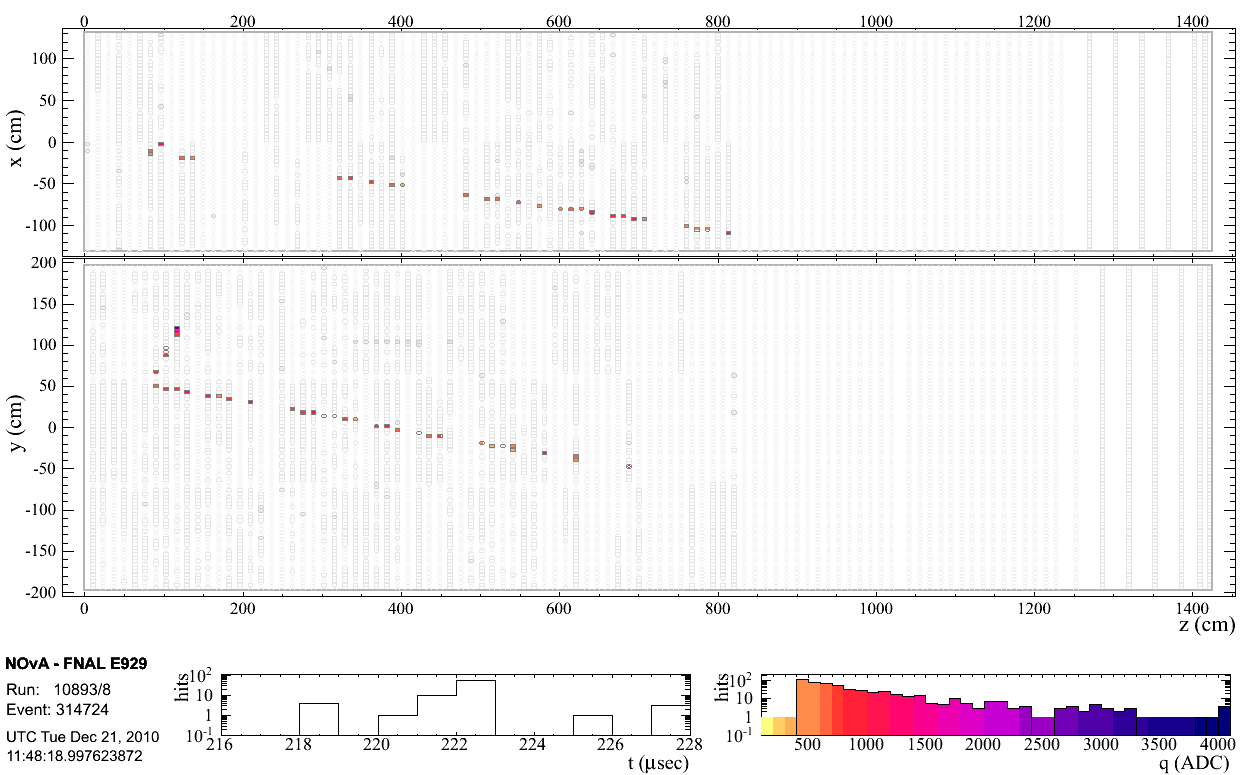
\includegraphics[width=\textwidth]{figures/evd/evd_ndos.png}
\end{center}
\caption{An example \nova event display.  The top projection is an $x$ vs. $z$ view, the bottom is $y$ vs. $z$.  This is a candidate \numu charged-current event from in NDOS.}
\label{eventDisplay}
\end{figure} 
Cells aligned side-by-side into units of 32 cells referred to as a modules.  Each cell is filled with scintillator-doped mineral oil to produce visible (blue) light in the presence of swiftly moving charged particles.  A strand of wavelength shifting (WLS) fiber runs up and down the length of each cell with both ends of fiber emerging at one end of the cell, visualized in Figure~\ref{cell}.  The fiber serves the purpose of capturing and transmitting the scintillation light in two steps; first by lengthening its wavelength through molecular absorption and reemission, and then trapping it within the fiber by total internal reflection.  At the end of the cells, photons trapped in the WLS fiber are converted to photoelectrons and multiplied in an avalanche photodiode (APD) to produce a measurable electrical signal.  One APD board contains 32 pixels to read out each cell of module separately.  The multiplied photoelectron signals are passed to an analog-to-digital converter (ADC) and written digitally to hard disk by a data concentrator module (DCM).  

The data acquisition system triggers on a \numi beam spill to record detector activity during time window centered on the beam spill.  Recorded activity can then be reviewed offline by custom computer software developed by collaborators to reconstruct physics events.  Physical quantities such as energy and momentum can then extracted for analysis.  Ultimately, this effort is rather similar to the analysis completed by the Brookhaven group that identified the muon neutrino; however, the data is collected and analyzed digitally rather than in a tracing lines on a photograph.  Data from the detector is visualized using a pair of orthogonal projections of the cell coordinates--- one projection for $x$ vs. $z$  and another for $y$ vs. $z$--- an example of which can be seen in Figure~\ref{eventDisplay}.  The analysis effort will be described in detail in the next section.  

\nova has installed and is collecting data with a prototype detector at Fermilab; this detector is known as the Near Detector on the Surface.  (NDOS)  Construction is underway for the Far Detector at Ash River and is anticipated to be complete in 2014; the Near Detector will be built in parallel with this effort to be completed within the same timeframe.  

\section{Physics Goals}
\label{goals}

It is expected that \nova will provide measurements of  \thetaoth and \thetatth.  Ideally, \nova will demonstrate agreement with Daya Bay and RENO regarding their nonzero measurement of \thetaoth.  It is also hoped that \nova will  hone the measurement of \thetatth to determine whether it is greater or less than $45^\circ$.  

Unique to accelerator neutrino experiments like \nova is the ability to produce either neutrinos or antineutrinos.  The matter effect, as described in section~\ref{matOsc}, predicts a difference between the appearance probabilities for neutrinos and antineutrinos.   By comparing the respective appearance probabilities, it could be possible to determine whether the mass hierarchy is normal or inverted.  The difference between neutrinos and antineutrinos could also be used to measure the CP violating phase, $\delta$.  

\section{Muon Neutrino Disappearance}

\nova and other long baseline experiments are configured such that \deltamtht, $L$ and $E$ combine to allow simplification to a two-flavor oscillation picture.  This replaces equation~\eqref{oscProbL} with:
\begin{equation}\label{muSurvProb}
P(\nu_\mu \rightarrow \nu_\mu) = 1 - \sin^2(2 \theta_{23})\sin^2 \bigg( 1.27 \frac{\Delta m^2_{32}[eV^2] L[km]}{E[GeV]} \bigg ), 
\end{equation}
written in units that are convenient for long baseline experiments.  The goal of a muon neutrino disappearance analysis is to measure the oscillation parameters \thetatth and \deltamtht. Determining these parameters is important not just for their own precision, but also to constrain errors in other other measurements such as \thetaoth, $\delta$ and the resolution of the mass hierarchy.  The analysis aims to observe a deficit in the \numu flux at the Far Detector relative to that measured at the Near Detector.  
\begin{figure}[h]
\begin{center}
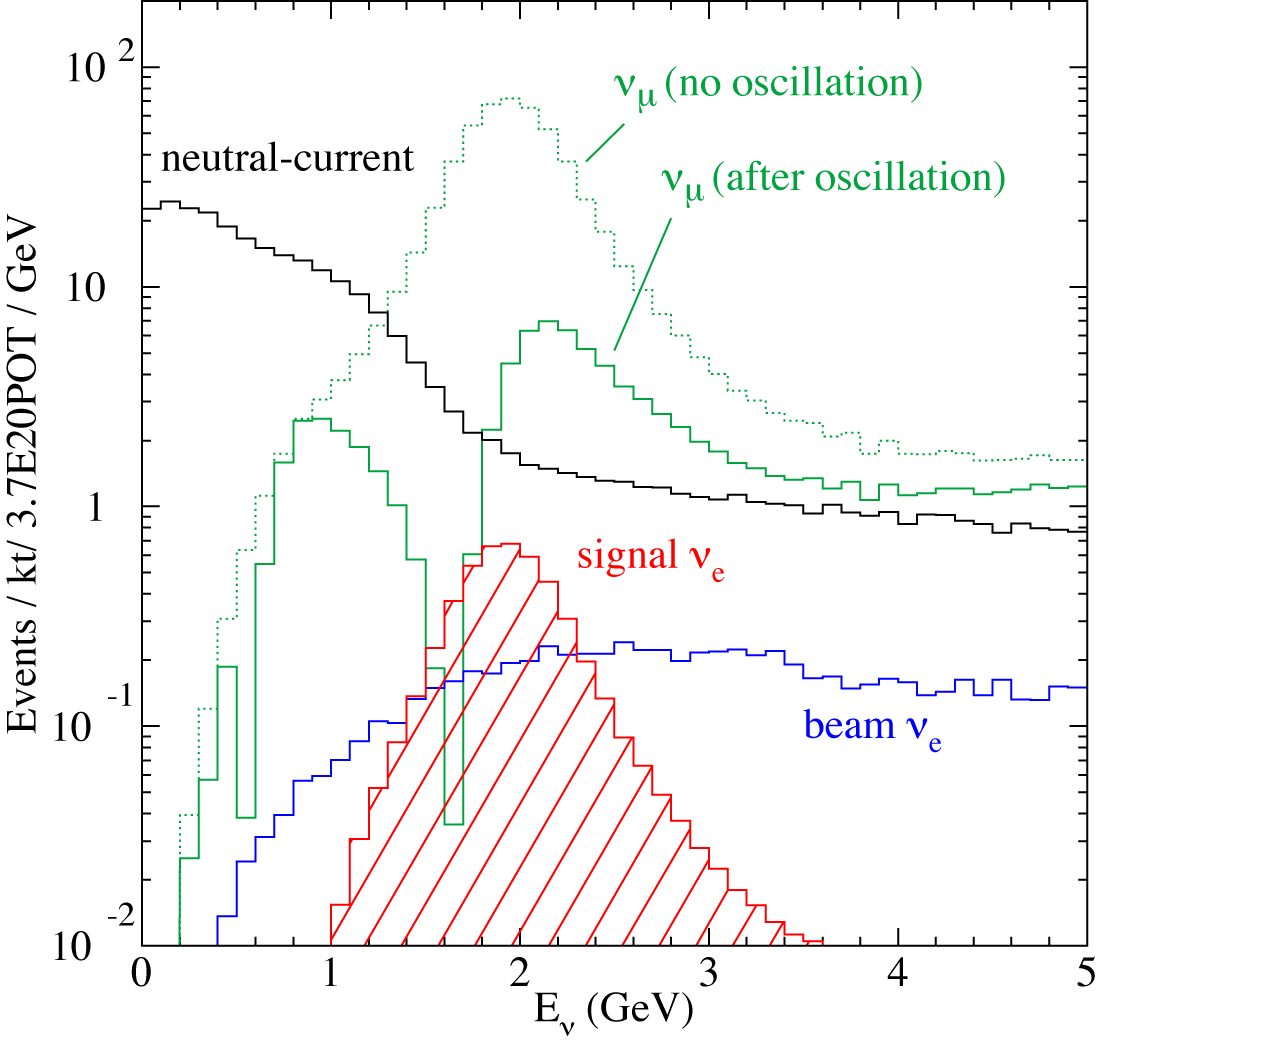
\includegraphics[width=0.75\textwidth]{figures/plots/nova/nuEventSpectrum.png}
\end{center}
\caption{The expected event spectrum at the \nova Far Detector.}
\label{spectrum}
\end{figure}
Figure~\ref{spectrum} demonstrates the deficit in expected event rate for particular interactions as a function of energy based on the expected beam flux and assuming best-fit measurements of \thetatth and \deltamtht.\cite{pdg}  The ultimate goal of the analysis is to fit the energy distribution of events in the far detector.  Detector activity must first be reconstructed, events must be selected and energies must be estimated; the following sections will outline this effort.



%%%%%%%%%%%%%%%%%%%%%%%%%%%%%%%%%%%%%%%%%%%%%%%%%%%%%%%%%%%%%%%%%%%%%%%%%%%%%%%%
